\section{Basics of Machine Learning}

\subsection{Some initial references}
Here are some resources that could help you for this next chapter:

\textbf{Books}:
\begin{itemize}
    \item \emph{Deep Learning Book} (Ian Goodfellow, Yoshua Bengio and Aaron Courville), \url{https://www.deeplearningbook.org/}
    \item \emph{The 100 pages ML book} (Andriy Burkov), \url{http://themlbook.com/wiki/doku.php}
    \item \emph{Deep Learning with Python} (Francois Chollet)
    \item \emph{The Elements of Statistical Learning} (Friedman, Tibshirani and Hastie)
\end{itemize}

\textbf{Online resources}:
\begin{itemize}
    \item Machine Learning Stanford Course: \url{https://cs229.stanford.edu/main_notes.pdf}
    \item Convolutional Neural Network for Visual Recognition, Stanford Course (also on YouTube): \url{https://cs231n.github.io/}
\end{itemize}

\textbf{Data Set}:
\begin{itemize}
    \item \url{https://www.cancerimagingarchive.net/}
    \item \url{https://www.kaggle.com/}
\end{itemize}


\subsection{Basic definitions and outline}

By \textbf{Artificial Intelligence (AI)}, we mean a set of techniques that rely on automatic learning by a machine to solve a complex and specific problem. 
\textbf{Machine Learning (ML)} is a vast field that includes many types of algorithms capable of learning to solve even very complex problems. 
In particular, \textbf{Deep learning (DL)} is machine learning made with \textbf{Deep Neural Networks (DNN)}, which we will learn to use in due time.

The basic idea is this: \textit{instead of producing rule-based algorithms we let the algorithm learn the rules}. Applications include for example autonomous driving, image and speech processing, agents able to play chess, play Go or drive cars, chatbots, anomaly detection (e.g. in credit card usage), and applications for research in various scientific fields (e.g. physics and medicine). For example, typical tasks include \textit{classification} (giving a discrete label to a certain type of data), \textit{segmentation} (assigning a class label to every fundamental unit of a data sample, such as a pixel in an image), \textit{regression} (predicting a continuous numerical output), \textit{super-resolution} (high-resolution image reconstruction from low-resolution images) and \textit{data generation} (creating new, synthetic data samples that resemble the original training distribution). 

%\includegraphics[width=0.8\textwidth]{lesson_ml_1_pag_4.png}

Here is a brief overview of the program we are going to follow in order to dive into the modern (and, in all fairness lucrative) world of machine learning:
\begin{enumerate}
    \item Introduction to basic concepts: 
    \begin{itemize}
        \item[-] Hypothesis function/Objective function
        \item[-] Training and inference
        \item[-] Learning paradigms (supervised, unsupervised and reinforcement) 
    \end{itemize}
    \item Supervised Learning:
    \begin{itemize}
        \item[-] Linear Regression
        \item[-] Logistic Regression (Cost function and optimization, Gradient Descent, Learning Rate).
    \end{itemize}
    \item Unsupervised learning: 
    \begin{itemize}
        \item[-] K-means algorithm
        \item[-] PCA
    \end{itemize} 
    \item Decision Tree.
    \item Capacity, underfitting, overfitting, bias-variance trade-off
    \item Regularization
    \item Data Management: 
    \begin{itemize}
        \item[-] Train/Validation/Test split
        \item[-] Cross-validation
        \item[-] Model selection
    \end{itemize} 
    \item Metrics
\end{enumerate}

\subsection{The hypothesis function and the 3 learning paradigms}
The goal of a ML algorithm is to approximate an unknown function (called hypothesis function $h(x)$ or often simply model) given some example data. If the output is continuous, we talk about \textbf{regression}; if the output is discrete, we talk about \textbf{classification}. In the figure below is a scheme that shows how a ML algorithm is built: we will dive deeper in all of its components.

\begin{center}
    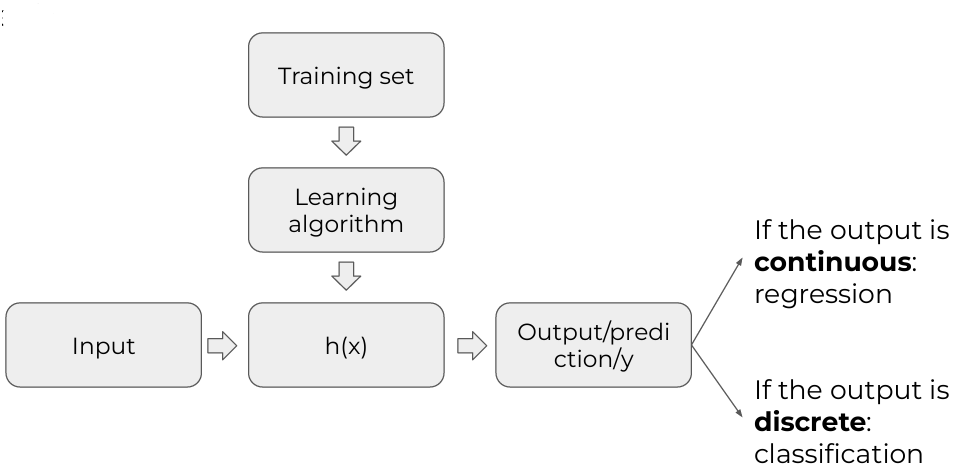
\includegraphics[width=0.8\textwidth]{figuresML/lesson_ml_1_pag_6.png}
\end{center}

We can distinguish two different phases in each ML algorithm:
\begin{itemize}
    \item[-] \textbf{Training phase} is the phase where the algorithm is allowed to change its parameters to learn how to approximate the function. We are going to call $\theta$ the parameters the model learns to solve the problem, i.e. to predict the correct output.
    \item[-] \textbf{Inference phase} is the test of a trained algorithm on unseen data. Of course, in this phase the algorithm cannot change its parameters.
\end{itemize}

There are thousands of learning algorithms, but each of them implements one of 3 types of \textbf{learning paradigms}:
\begin{itemize}
    \item[-] \textbf{Supervised}: Many inputs or \textbf{features} ($x$) associated with their \textbf{targets} ($y$, often referred to as \textit{labels} or \textbf{ground truth}) are given to the algorithm. We call "example" each $(x^{(i)},y^{(i)})$ couple, since $y$ represents the expected output given the input $x$ of the function $h$ we are trying to approximate. The algorithm has to find the underlying connections between data that solve a specified task, i.e. to find the best parameters for $h$.
    \item[-] \textbf{Unsupervised}: Many training samples ($x$) without a specific label are used to train the algorithm. The algorithm should learn to discover patterns, groupings, and relationships within the data without explicit guidance or prior knowledge of the desired outcomes. This paradigm can be much more difficult to implement with respect to the supervised one, since in this case we are forced to make stronger assumptions for weaker guarantees. The upside is that we are probably going to get much more information out of our dataset, since it can be used even if we do not have the "answers" to feed to the agent during training.
    \item[-] \textbf{Reinforcement}: In the reinforcement learning framework, we provide our algorithms only a \textit{reward function}, which indicates to the learning agent when it is doing well, and/or a penalty when it is doing poorly. This is the learning paradigm used to teach an algorithm to play chess or GO.
\end{itemize}

We will mainly focus our attention on supervised and unsupervised algorithms.

\subsection{Supervised learning: Gradient descent methods for regression}
We are going to go through a simple case of supervised learning in order to understand its basic principles. 

Let $d$ be the number of features and $n$ the number of training examples, so that our training set is a set of examples $(x, y)$. 
Assume that our hypothesis function is that input and output (continuous) are linearly related:
\begin{equation}
h(x) = \sum_{j=0}^{d} \theta_{j} x_{j}
\end{equation}
As said, training means finding the parameters $\theta$ that better fit the data $x$. 

We want to choose $\theta$ such that $h(x) \approx y$ for the training examples. To achieve this, we need to define a \textbf{cost function} (or loss function) which basically tells us how far our approximation is from the correct answer. In this case, we choose the \textit{mean squared error}:
\begin{equation}
J(\theta) = \frac{1}{2n}\sum_{i=1}^{n}(h_{\theta}(x^{(i)}) - y^{(i)})^{2}
\end{equation}
This kind of problem should look familiar: we are just implementing the ordinary \textit{least squares method} for \textit{linear regression}. However, the choice of the loss function depends on the kind of the problem. For instance...
\begin{itemize}
    \item[-] ... if we have a classification task we can use the so called \textit{Binary Cross Entropy}: 
    \begin{equation*}
        D_{BCE}(y,\hat{y}) = -\frac{1}{N}\sum_{i=1}^{N}[y_{i}\log(\hat{y}_{i}) + (1-y_{i})\log(1-\hat{y}_{i})]
    \end{equation*}
    \item[-] ... if we have a segmentation task we can use the so called \textit{Dice Loss}: 
    \begin{equation*}
        DSC_{loss} = 1 - 2\frac{|X \cap Y|}{|X \cup Y|}
    \end{equation*}
\end{itemize}
Whatever loss function we are using the goal is always the same: we need to \textbf{minimize it}.

We start with random parameters ($\theta_{random}$) and keep changing $\theta$ to reduce the cost function $J(\theta)$. Considering a fixed dataset, implementing a \textbf{Gradient Descent (GD) algorithm} means updating the parameters following this rule:
\begin{equation}
\theta_{j} := \theta_{j} - \alpha \frac{\partial J(\theta)}{\partial\theta_{j}} \quad \text{for } j=0,...,d
\end{equation}
This formula means that we take the old value of the parameter $\theta_j$ and modify it towards the direction where the gradient of the error function is steeper. With the help of the following figure you can already note a fundamental problem: depending on the initialization parameters we could reach different minimums every time. 

\begin{center}
    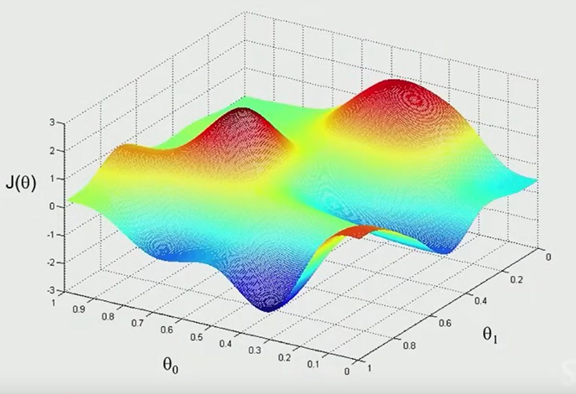
\includegraphics[width=0.6\textwidth]{figuresML/lesson_ml_1_pag_17.png}
\end{center}

The parameter $\alpha$ is called \textbf{Learning Rate (LR)} and it is actually a hyperparameter: parameters ($\theta$) change during training, while hyperparameters include all the choices made by the programmer that cannot be learnt by the algorithm. The "length of the step" we make in one iteration is given by the value of the learning rate.
Here is a pivotal fact: \textbf{the wrongful choice of the learning rate can break your learning algorithm}. Take a look at the following figure. Note that:
\begin{itemize}
    \item[-] if you choose a low value for $\alpha$, the process will be slow and you will need a lot of computational power in order to reach a minimum;
    \item[-] if you choose a high value for $\alpha$, you might not reach the minimum at all given the fact that your "steps" might be so long that your algorithm might start to oscillate, just as in this figure.
\end{itemize}
One of the best ways to decide the learning rate is an \textit{adaptive way: while the loss is approaching the minimum, we decrease the learning rate!}

\begin{center}
    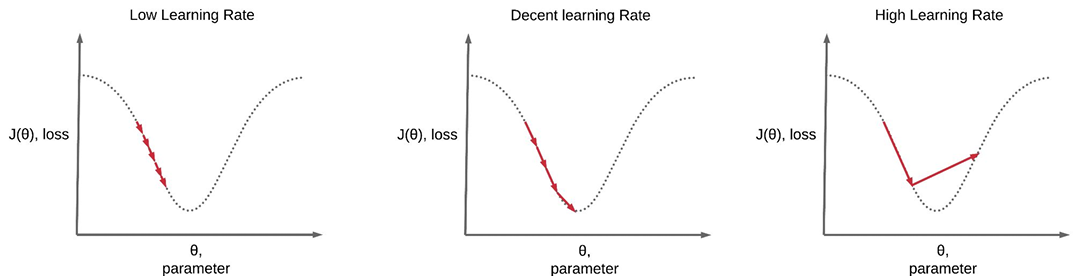
\includegraphics[width=0.69\textwidth]{figuresML/lesson_ml_1_pag_20.png} $\ \rightarrow \ $
    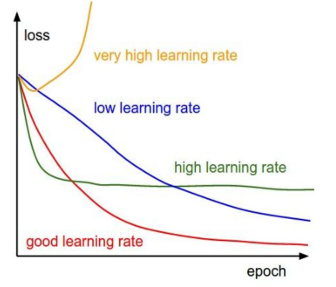
\includegraphics[width=0.23\textwidth]{figuresML/lesson_ml_1_pag_21.png}
\end{center}

If we go back to our example for a second, we see that we can compute the partial derivative of $J$ with respect to $\theta_j$ in the case of linear regression and squared error:
\begin{equation}
\theta_{j} := \theta_{j} + \alpha\frac{1}{n}\sum_{i=1}^{n}(y^{(i)} - h_{\theta}(x^{(i)}))x_{j}^{(i)}
\end{equation}

The method underlined in the last few paragraphs looks at every example in the entire training set on every step and it is called \textbf{Batch Gradient Descent (BGD)} or simply \textbf{Gradient Descent (BGD)}. There is an alternative called the \textbf{Stochastic Gradient Descent (SGD)} which, instead of using all the training examples, uses only one of them and makes the upgrade. The SGD has many drawbacks such as:
\begin{itemize}
    \item[-] it is prone to converge to local optima;
    \item[-] may get trapped in saddle points in certain cases;
    \item[-] it makes it difficult to choose a suitable learning rate;
    \item[-] all parameters use the same learning rate.
\end{itemize}
The most used method nowadays (practically the default if possible) is the so called \textbf{Mini-batch SGD}: instead of using all the input data or only one, we use a bunch of them and then we average the gradients.

\subsection{Supervised learning: Binary classification in a probabilistic approach}

In a \textit{binary classification} task, the goal is to categorize data into one of two mutually exclusive classes. By convention, these classes are mathematically represented as $y \in \{0, 1\}$. For example you might want to determine whether an email is spam ($1$) or not ($0$), or whether a medical tumour is malignant ($1$) or benign ($0$).

You might have thought to apply our previous linear regression model, $h(x) = \theta^{T}x$, and simply set a threshold to separate the classes. However, this approach is fundamentally flawed since the output of a linear combination can range from $-\infty$ to $+\infty$, whereas we want to interpret our hypothesis as the \textit{probability} that an example belongs to the positive class. By definition, probabilities must be strictly bounded in the $[0, 1]$ interval. To achieve this, we need to change our hypothesis function to the \textbf{sigmoid (or logistic) function}:
\begin{equation}
    h_{\theta}(x) = g(\theta^{T}x) = \frac{1}{1+e^{-\theta^{T}x}}
\end{equation}
The derivative of the sigmoid is nice because it is equal to: $g^{\prime}(z) = g(z)(1-g(z))$.

\begin{center}
    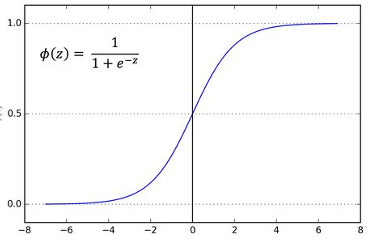
\includegraphics[width=0.4\textwidth]{figuresML/lesson_ml_1_pag_24.png}
\end{center}

Let's assume that $p(y=1|x;\theta) = h_{\theta}(x)$ and $p(y=0|x;\theta) = 1-h_{\theta}(x)$. We can write this more compactly as: 
\begin{equation}
p(y|x;\theta) = (h_{\theta}(x))^{y}(1-h_{\theta}(x))^{1-y}
\end{equation}
Assuming that the $n$ training examples were generated independently, we can write the so called \textbf{Likelihood} function:
\begin{equation}
L(\theta) = p(\vec{y}|x;\theta) = \prod_{i=1}^{n} (h_{\theta}(x^{(i)}))^{y^{(i)}} (1-h_{\theta}(x^{(i)}))^{1-y^{(i)}}
\end{equation}
The likelihood is the probability of observing the data conditioned by the parameters $\theta$. This is just another way to proceed: instead of defining a loss function to minimize (which you can also do), here we just use a likelihood that of course needs to be maximized.

For computational efficiency we can maximize a strictly increasing function of the likelihood, like its $\log$:
\begin{equation}
l(\theta) = \log L(\theta) = \sum_{i=1}^{n} y^{(i)}\log h(x^{(i)}) + (1-y^{(i)})\log(1-h(x^{(i)}))
\end{equation}
Now, we have to maximize it via gradient ascent just like before:
\begin{equation*}
\dfrac{\partial l}{\partial \theta_j}= ... = \sum_{i=1}^{n}(y^{(i)}-h_\theta (x^{(i)}))x^{(i)}_j \quad \Rightarrow
\end{equation*}
\begin{equation}
\theta_{j} := \theta_{j} + \alpha\sum_{i=1}^{n}(y^{(i)} - h_{\theta}(x^{(i)}))x_{j}^{(i)}
\end{equation}

\subsection{Unsupervised learning: K-means}

In this scenario, we do not have any label, we see only our inputs/points. We assume that there exists a latent or hidden structure inside the input data. The question is: can I recover it? 
The kind of problems we can solve with this approach are:
\begin{enumerate}
    \item Classification of "common'' patterns (clustering)
    \item Dimensionality reduction, compression
    \item Prediction of missing inputs
    \item Anomaly detection
\end{enumerate}

\begin{figure}[H]
    \begin{minipage}[c]{0.55\textwidth}
    Let's suppose we want to perform a clustering of input data $x^{(1)},...,x^{(n)} \in \mathbb{R}^{d}$ and $k$ is the number of clusters. We must find an assignment of points to clusters $C^{(i)}=j$ assuming that each point belongs only to one cluster. Note that one of the main problems with this approach could be defining the number $k$ itself. One way to do that is using the so called \textbf{K-means} algorithm:
    \begin{enumerate}
        \item Randomly initialize point centers $\mu^{(1)}, \dots, \mu^{(k)}$.
        \item Define a distance and assign each point to a cluster following the rule \\ $C^{(i)} = \text{argmin}_{j} (||\mu^{(j)} - x^{(i)}||)$.
        \item Compute new cluster centers as the mean of the positions of the points of the clusters.
        \item Repeat until convergence, that is when centers points do not change between different iterations.
\end{enumerate}
    \end{minipage}\hfill 
    \begin{minipage}[c]{0.4\textwidth}
        \centering
        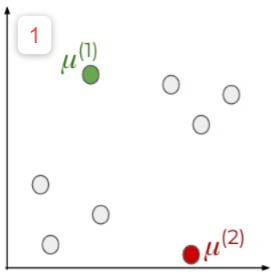
\includegraphics[width=0.48\linewidth]{figuresML/lesson_ml_1_pag_30.png}\hfill
        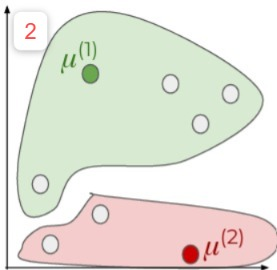
\includegraphics[width=0.48\linewidth]{figuresML/lesson_ml_1_pag_31.png} \\[.25cm] 
        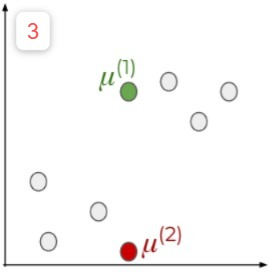
\includegraphics[width=0.48\linewidth]{figuresML/lesson_ml_1_pag_32.png}\hfill
        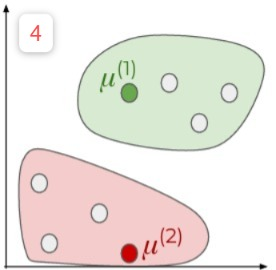
\includegraphics[width=0.48\linewidth]{figuresML/lesson_ml_1_pag_33.png}
    \end{minipage}
\end{figure} 

\subsection{Unsupervised learning: Principal Component Analysis (PCA)}
The so called \textbf{Principal Component Analysis (PCA)} algorithm is used for dimensionality reduction (which is pivotal since it may happen that you have more features than samples in your data) to simplify complex datasets. PCA aims to find new variables (called \textbf{principal components}) that are linear combinations of the original variables. These new variables are orthogonal (uncorrelated) and capture the maximum possible variance in the data.

Here's how PCA works:
\begin{enumerate}
    \item \textit{Data Standardization}: each variable is centered (by subtracting the mean) and scaled (by dividing for the standard deviation).
    \item \textit{Covariance Matrix Computation}: Compute the covariance matrix which captures how the variables vary together: $\Sigma = \frac{1}{1-N} X^{T}X$.
    \item \textit{Eigenvalue and Eigenvector Computation}: The eigenvectors of the covariance matrix define the directions of the principal components, while the eigenvalues indicate how much variance is explained by each of them.
    \item \textit{Selection of Principal Components}: The first $k$ components that explain the most variance are selected, as represented in the following figure. $k$ must be chosen wisely: if $k$ is too low we might not be able to solve our task, if it is too high you might end up using a lot of computational power. 
    \item \textit{Data Projection}: the original data is projected onto the space defined by the selected components, resulting in a dataset with fewer dimensions.
\end{enumerate}

\begin{center}
    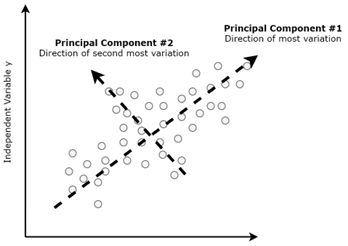
\includegraphics[width=0.35\textwidth]{figuresML/lesson_ml_1_pag_34.png}
\end{center}

\subsection{Supervised learning: $k$-Nearest neighbors}

The \textbf{$k$-Nearest Neighbors (kNN)} algorithm is a very powerful, instance-based method used for both classification and regression tasks. Unlike other algorithms that learn an explicit internal model during the training phase, kNN is considered a "lazy learner." Its core mechanism involves evaluating a new, unseen sample by looking at the data points in the training dataset that are \textit{close} to the sample itself in the feature space.

Here is how the algorithm generally operates:
\begin{itemize}
    \item[-] We choose a parameter \textbf{$k$}, which represents the number of neighbors.
    \item[-] We compute the distance between the new sample and all the points in the training set.
    \item[-] We look at the $k$ closest samples.
    \item[-] The final prediction is then made based on these neighbors (e.g., by a majority vote for classification, or by averaging the targets for regression).
\end{itemize}

Multiple neighbors ($k > 1$) can be used for a more stable evaluation, as it makes the algorithm's predictions less sensitive to noise or outliers in the training data. However, this approach comes with a significant drawback: on large datasets, it could be a major computational and memory problem to keep all training points available and calculate distances against them during the evaluation phase.

While they both rely on spatial distance, kNN and K-means serve entirely different purposes and belong to different learning paradigms:
\begin{itemize}
    \item[-] \textbf{kNN} is a \textit{supervised learning} algorithm. It relies on a completely labeled training dataset to predict the specific class or continuous target of a new, individual data point.
    \item[-] \textbf{K-means}, as discussed in the previous sections, is an \textit{unsupervised learning} algorithm. It operates on completely unlabeled data with the goal of discovering hidden structures, partitioning the entire dataset into $K$ distinct clusters.
\end{itemize}

\subsection{Another way to classify data: Decision Trees}
A \textbf{decision tree} is a predictive model, where leaves represent class labels and branches represent conjunctions of features that lead to those class labels. It is very hard to solve some problems with a linear model. Take a look at the example below which contains 2 classes (negative and positive) of points in a 2 dimensional feature space ($x_1 \in [0,12]$, $x_2 \in [-90, 90]$): it is clear that linear regression and clustering will not work for our classification task.

\begin{center}
    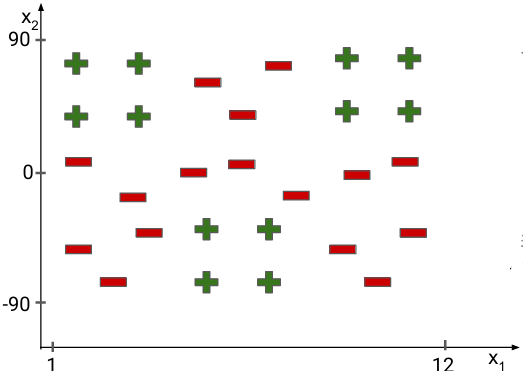
\includegraphics[width=0.35\textwidth]{figuresML/lesson_ml_1_pag_36.png}
\end{center}

Now we should try to isolate a cluster of negatives (a \textbf{leaf}) by imposing some conditions on $x_1$ and $x_2$ (\textbf{nodes}). The "tree" structure appears as a sequence of choices (which define the \textbf{branches}) is made until convergence is reached, as shown below. 

\begin{center}
    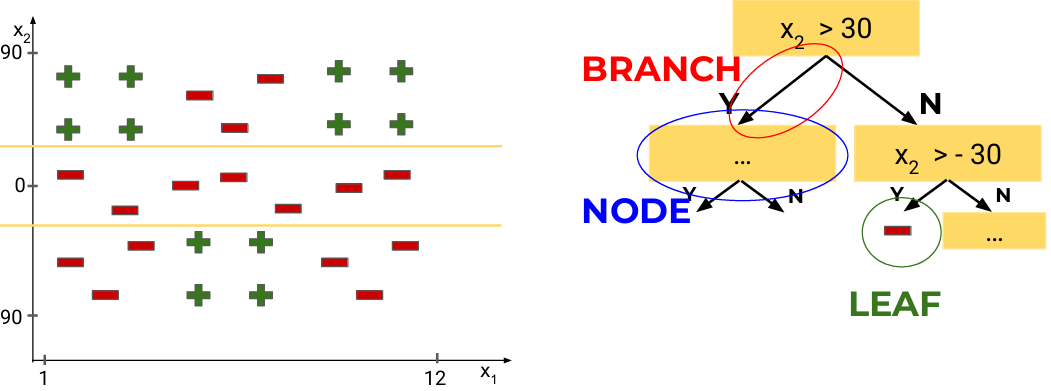
\includegraphics[width=0.6\textwidth]{figuresML/lesson_ml_1_pag_40.png}
\end{center}

More rigorously, we look for the \textbf{split function} $S_{p}(j,t)$ where $j$ is the $j$-th feature and $t$ is the threshold to partition the parent region $R_{p}$:
\begin{equation}
S_{p}(j,t) = ( \{x \ | \ x_{j} < t, x \in R_{p}\} \ , \ \{x \ | \ x_{j} \ge t, x \in R_{p}\} )
\end{equation}
Our objective is reaching \textbf{purity}: we want that at the end of the training, each leaf contains only one class. \\ Given the class $c$, we define $\hat{p}_{c}$ to be the proportion of class k observations (with N observations) in node $m$:
\begin{equation}
\hat{p}_{c} = \frac{1}{N}\sum_{x_{i} \in R_{m}} I(y_{i}=c)
\end{equation}
We then define an impurity measure which gives us an idea of the relative number of points that have been misclassified at each node. For example, we could choose the \textbf{misclassification loss}
\begin{equation}
L_{misclass} = 1 - \max(\hat{p}_{c}) \quad \text{,}
\end{equation}
but we rapidly run into an issue. Take a look at the two different splits below. In the first example the $R_1$ and $R_2$ nodes still contain both - and + values, while in the second one $R_2$ is already a leaf. It should be obvious that the latter is the better choice. However if we compute the weighted mean misclassification loss we get the same value for the two cases: 
\begin{equation*}
\begin{aligned}
    L_1 &= \frac{N_1}{N} L(R_1) + \frac{N_2}{N} L(R_2) = \frac{400}{800}\left(1-\frac{300}{400}\right) + \frac{400}{800}\left(1-\frac{300}{400}\right) = 0.25 \\ 
    L_2 &= \frac{N_1}{N} L(R_1) + \frac{N_2}{N} L(R_2) = \frac{600}{800}\left(1-\frac{400}{600}\right) + \frac{200}{800}\left(1-\frac{200}{200}\right) = 0.25
\end{aligned}
\end{equation*}
\begin{center}
    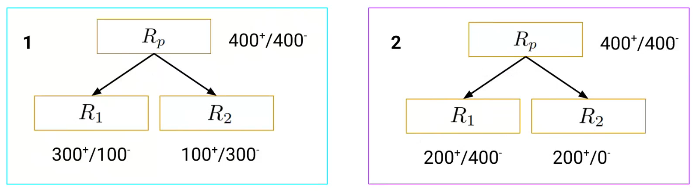
\includegraphics[width=0.6\textwidth]{figuresML/lesson_ml_1_pag_42.png}
\end{center}
We can then use another type of impurity measure, such as the \textbf{Cross-Entropy} 
\begin{equation}
    L_{CE} = -\sum_{c}\hat{p}_{c}\log\hat{p}_{c} 
\end{equation} 
or the \textbf{Gini impurity} 
\begin{equation}
    G = 1 - \sum_{i=1}^{C}p_{i}^{2}
\end{equation} 
Applying the latter in the previous example we get
\begin{equation}
\begin{aligned}
    G_{1} &= \frac{N_1}{N} G(R_1) + \frac{N_2}{N} G(R_2) \\
           &= \frac{400}{800}\left[1-\left(\frac{300}{400}\right)^2-\left(\frac{100}{400}\right)^2\right] + \frac{400}{800}\left[1-\left(\frac{100}{400}\right)^2-\left(\frac{300}{400}\right)^2\right] = 0.375 \\ 
    G_{2} &= \frac{N_1}{N} G(R_1) + \frac{N_2}{N} G(R_2) \\
           &= \frac{600}{800}\left[1-\left(\frac{400}{600}\right)^2-\left(\frac{200}{600}\right)^2\right] + \frac{200}{800}\left[1-\left(\frac{200}{200}\right)^2-\left(\frac{0}{200}\right)^2\right] = 0.333
\end{aligned}
\end{equation}
When computing a decision tree, we compute all the possible impurities in every possible split in order to choose the most efficient way to reach convergence, similarly to the gradient descent method. To sum up, decision trees are easy to explain, interpretable, fast and can handle categorical variables. However they usually have a low predictive accuracy and high variance and of course they are not additive. 

\hrulefill
\\ Note: Scikit-learn library offers many ML techniques implementation in Python. You can find it here: \url{https://scikit-learn.org/stable/index.html}. Here's a representation of different classification methods implemented using this library. 
\begin{center}
    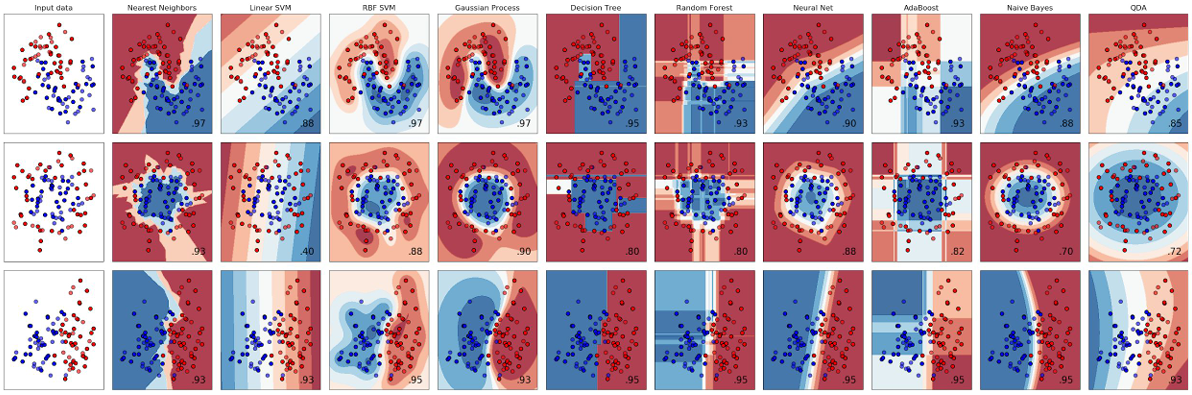
\includegraphics[width=0.9\textwidth]{figuresML/lesson_ml_1_pag_48.png}
\end{center}
\hrulefill

\subsection{Representational learning and Capacity}

Before diving into more complex architectures like Neural Networks, it is crucial to observe the learning process from a more holistic point of view. When we define a specific hypothesis function, we are essentially declaring how we choose to represent our data and our problem (e.g., framing it as a classification task). This "representation" is fundamentally driven by two main factors: the available data and the specific type of algorithm we select.

We can distinguish between two major paradigms based on how this representation is constructed:
\begin{itemize}
    \item[-] \textit{Classical Machine Learning}: In traditional models, the representation heavily relies on human intervention (often referred to as \textit{Feature Engineering}). The algorithm's performance depends on how we manually compute and extract input features or measures from the raw data. For instance, if dealing with a raw time-domain signal, a physicist might first apply a Fourier transform to pass only the relevant frequency amplitudes to a linear classifier. Furthermore, the representation depends on the intrinsic complexity of the chosen mathematical model (e.g., choosing a polynomial model of degree $d$ versus a purely linear one) and its number of free parameters.
    \item[-] \textbf{Deep Learning (Representational Learning)}: In this paradigm, the optimal representation is learned directly and automatically by the model itself. Instead of manually engineering features, we feed raw data to the algorithm and let the training process discover the most useful mathematical transformations to solve the specific problem. A classic example is a Convolutional Neural Network (CNN): we input raw image pixels, and the network learns to represent them hierarchically. It might learn to detect simple edges in its first layers, combine them into shapes in intermediate layers, and finally recognize complex objects in the deepest layers. As with classical ML, the capacity of this learned representation still depends on the number of free parameters available to the network.
\end{itemize}

Different models can represent different types of function, and of course models with more parameters can approximate a larger number of functions. The ability of representing many functions is called \textbf{capacity}, which measures the model's ability to use information effectively (e.g. in a Neural Network: more neurons, more layers $\to$ greater capacity).

With that said, the choice seems simple enough: you should just use the model with the highest capacity to fit the data precisely. Unfortunately, that is horrendously wrong. Our goal is not simply to fit the training data, but to make the algorithm work on unseen ones. In fact, by increasing the number of parameters one could theoretically fit a function for any kind of dataset. The ability of a model to have good performance on unseen data is called \textbf{generalization capability}. 

Take a look at the following figure witch represents a polynomial fitting:
\begin{itemize}
    \item[-] In the first panel the dataset is not fitted properly since the grade of the chosen polynomial is too low. It is a classical case of \textbf{underfitting}.
    \item[-] In the second panel the dataset is perfectly fitted.
    \item[-] In the third panel the dataset is fitted using a high number of parameters: the algorithm has "learned by heart" the training data and it won't work with other samples. We are looking at \textbf{overfitting}
\end{itemize} 

\begin{center}
    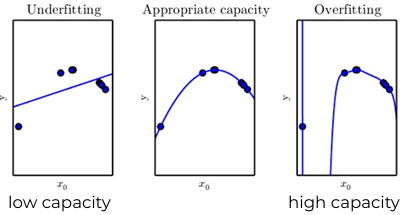
\includegraphics[width=0.4\textwidth]{figuresML/lesson_ml_1_pag_52.png}
\end{center}

The problem is that you will need to program algorithms with millions of parameters and in those cases is not as easy to spot overfitting problems, but there are many methods to try and avoid it. For example, it is standard procedure to split our dataset in a training set and a validation set. We train the algorithm using the first one and then confront its predictions with the validation set, as shown here. 

\begin{center}
    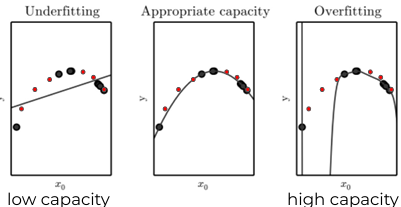
\includegraphics[width=0.4\textwidth]{figuresML/lesson_ml_1_pag_54.png}
\end{center}

Another practical tip when developing very complex models is to start in an underfitting situation and then add parameters until you get out of it. 

Before you go on, make sure that you understood the non trivial link between capacity and generalization.

\subsection{Regularization}
There exist some techniques that help in achieving good performance on data different from the training set even with a high number of parameters known as \textbf{regularization techniques}. Different algorithms need to be regularized in different methods, but many mechanisms can be implemented to the vast majority of them. \\ 
Here are the most common and practical ways:
\begin{itemize}
    \item[-] The cost function can be modified by adding regularization terms
    \item[-] The examples in the training dataset can be increased with \textbf{augmentation techniques}.
    \item[-] \textit{Stochastic noise} can be added to the data.
    \item[-] Existing examples can be transformed with transformations that are known to be invariant for the solution we look for. 
\end{itemize}
One of the most common practice is adding a \textbf{penalty} to the loss function in order to limit some parts of the model parameter space. \\
However, you should be aware of the risks of doing so. Take a look at the following example where we are fitting data using a 5 degrees polynomial $\theta_0 + \theta_1x +...+\theta_5x^5$. The loss function $J(\theta)$ is modified to be $J(\theta) + \sqrt{\lambda||\theta||^{2}}$. As you can see, when $\lambda$ is set to a high value, the easiest way to minimize such function is to set all the parameters $\theta$ to zero, which obviously ruins our fit.

\begin{center}
    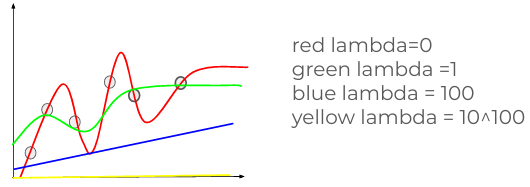
\includegraphics[width=0.55\textwidth]{figuresML/lesson_ml_1_pag_59.png}
\end{center}

\subsection{Data management for model selection}

As mentioned before, we need an intelligent way to divide and use our dataset. A standard practice is dividing the available data into three distinct subsets:
\begin{itemize}
    \item \textbf{Training set}: used for algorithm training and fitting the model's parameters.
    \item \textbf{Validation set}: used to test the algorithm during the training phase, allowing for model selection and tuning without biasing the final evaluation.
    \item \textbf{Test set}: strictly reserved to test the final algorithm's performance on unseen data.
\end{itemize}

An alternative and robust approach is \textbf{K-Fold Cross validation}, which involves dividing the data into multiple folds and iteratively using different combinations of them as training and test data, as shown in the figure below. Variations of this method include \textit{Stratified cross validation} and \textit{Nested Stratified cross validation}.

\begin{center}
    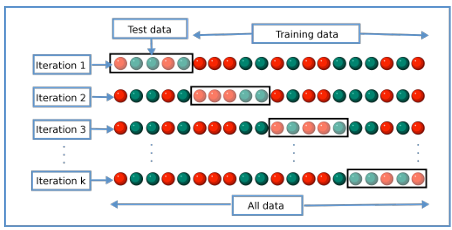
\includegraphics[width=0.7\textwidth]{figuresML/lesson_ml_1_pag_60.png}
\end{center}

\subsection{Hyperparameters optimization}
We have seen that models rely on different hyperparameters. When we develop complex architectures like a Neural Network, we will have many hyperparameters to tune. To search for the best configuration, two common strategies are used (as shown below):
\begin{itemize}
    \item[-] \textbf{Grid Search}: exhaustively evaluating a predefined, regular grid of hyperparameter values.
    \item[-] \textbf{Random Search}: sampling hyperparameter combinations randomly within defined distributions.
\end{itemize}

\begin{center}
    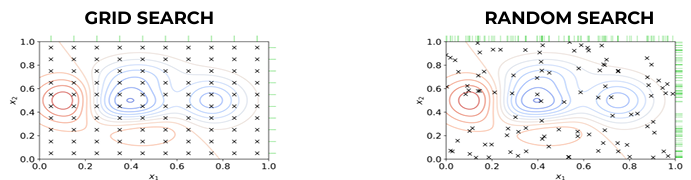
\includegraphics[width=0.85\textwidth]{figuresML/lesson_ml_1_pag_61.png}
\end{center}

\subsection{Metrics}
In the context of machine learning, a \textbf{metric} is a quantifiable measure used to evaluate the performance of a model. While a loss function is used internally by the algorithm during the training phase to update its parameters, a metric is primarily used by developers to interpret how well the model is performing and generalizing on the data (especially on the validation and test sets). It provides a mathematical way to compare the model's predictions against the actual ground truth.

The metric to be used strictly depends on the problem we want to solve and on the distribution of our data.
\begin{itemize}
    \item \textit{Regression}: common metrics include 
    \begin{itemize}
        \item[-] MAE (Mean Absolute Error);
        \item[-] MSE (Mean Squared Error);
        \item[-] RMSE (Root Mean Squared Error).
    \end{itemize}    
    \item \textit{Classification}: common metrics include 
    \begin{itemize}
        \item[-] Accuracy (proportion of correct predictions);
        \item[-] Precision (proportion of true positives among predicted positives);
        \item[-] Recall (or sensitivity, proportion of true positives among actual positives);
        \item[-] F1-score (the harmonic mean of precision and recall);
        \item[-] ROC-AUC (area under the ROC curve for binary classification);
        \item[-] Confusion Matrix (showing TP, FP, FN, TN, see below).
    \end{itemize}
    \item \textit{Segmentation}: common metrics include
    \begin{itemize}
        \item[-] IoU (Intersection over Union, overlap between predicted and true regions);
        \item[-] Dice Coefficient (overlap measure similar to F1 score);
        \item[-] Pixel Accuracy (percentage of correctly classified pixels);
        \item[-] Mean IoU (average IoU across all classes).
    \end{itemize}
\end{itemize}
It is beyond this course to focus on each and everyone of those, but let's look at some important examples.

For a \textit{binary classification} task, the predictions can be summarized in a so called \textbf{Confusion Matrix} comparing the predicted class with the true class (positive or negative). The matrix elements are:
\begin{itemize}
    \item[-] True Positive (TP): correctly predicted positive.
    \item[-] False Negative (FN): incorrectly predicted negative.
    \item[-] False Positive (FP): incorrectly predicted positive.
    \item[-] True Negative (TN): correctly predicted negative.
\end{itemize}
From these, several important metrics can be derived, as shown in the following figure.

\begin{center}
    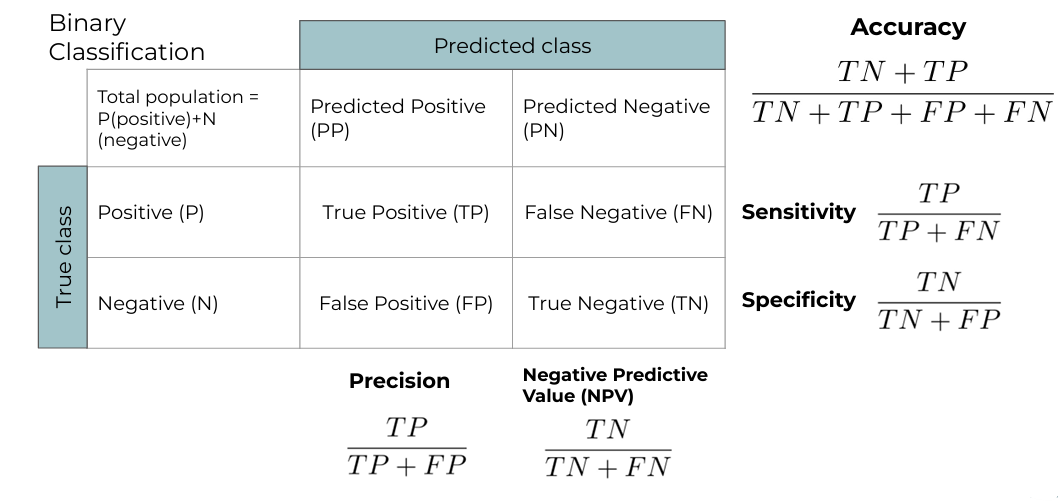
\includegraphics[width=0.85\textwidth]{figuresML/lesson_ml_1_pag_63.png}
\end{center}

For multi-class classification tasks, this concept is naturally extended into a larger, multi-class confusion matrix where the diagonal represents correct predictions.

\begin{center}
    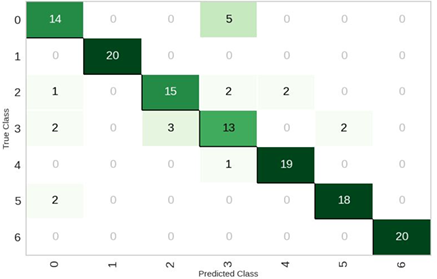
\includegraphics[width=0.55\textwidth]{figuresML/lesson_ml_1_pag_65.png}
\end{center}

We can interpret the output of a classifier as a class probability (this is always true in binary classification, while it depends in multi-class scenarios). The \textbf{ROC curve} (figure below) is constructed by plotting the True positive rate ($\frac{TP}{P}$) on the y-axis against the False positive rate ($\frac{FP}{N}$) on the x-axis for every possible classification threshold. 
\begin{center}
    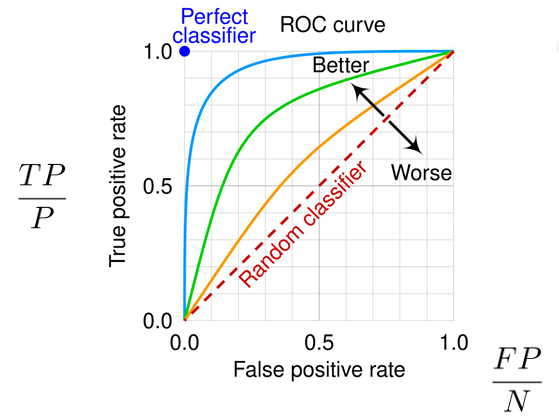
\includegraphics[width=0.45\textwidth]{figuresML/lesson_ml_1_pag_64.png}
\end{center}
To summarize the overall performance of the model into a single scalar value, we compute the \textit{AUC} (Area Under the Curve). The AUC evaluates how well the model can distinguish between classes, regardless of the specific threshold chosen. 
\begin{itemize}
    \item[-] AUC = 1.0: Perfect classifier.
    \item[-] AUC = 0.5: Random classifier (represented by the diagonal line).
\end{itemize}
Probabilistically, the AUC represents the probability that the model will rank a randomly chosen positive instance higher than a randomly chosen negative one. This metric is extremely robust and heavily used in fields like medicine.

For segmentation tasks, evaluating performance pixel-by-pixel can be misleading (as we will see in the prevalence problem). Instead, we often rely on \textbf{overlap measures}. An overlap measure quantifies the spatial agreement between the predicted segmentation mask ($X$) and the ground truth mask ($Y$). Rather than just counting correctly classified pixels, these metrics evaluate how well the shape, size, and position of the predicted object match the real one.

The two most common overlap measures are:
\begin{itemize}
    \item[-] \textbf{Intersection over Union (IoU)} (also known as the Jaccard Index): This metric calculates the area of overlap between the prediction and the ground truth, divided by the total area covered by both combined (their union). It is a strict metric that evaluates the overall spatial correspondence and heavily penalizes both false positives and false negatives.
    $$IoU = \frac{|X \cap Y|}{|X \cup Y|}$$
    
    \item[-] \textbf{Dice Similarity Coefficient (DSC)} (or Dice index): This metric is essentially the F1-score applied to spatial data. It doubles the intersection area and divides it by the sum of the total areas of both masks. While very similar to IoU and perfectly correlated, DSC tends to give slightly more weight to the correctly predicted pixels (the intersection), often resulting in a slightly higher score than IoU for the same prediction.
    $$DSC = \frac{2|X \cap Y|}{|X| + |Y|}$$
\end{itemize}

\textit{Exercise: try to write these two metrics in terms of TP, FP and FN}. \\
Let's solve this exercise to better understand how these metrics relate to the standard confusion matrix. If we consider the overlapping region $X \cap Y$ as the True Positives (TP), the remaining part of the predicted mask as False Positives (FP), and the unpredicted part of the ground truth mask as False Negatives (FN), we can rewrite the formulas as follows:
$$ IoU = \frac{TP}{TP + FP + FN} $$
$$ DSC = \frac{2TP}{2TP + FP + FN} $$

It should be clear that using the wrong metric can be highly deceiving. Here are two cases showing, for example, why accuracy is not always the optimal choice:
\begin{enumerate}
    \item Let's suppose we are solving a binary classification task and our test set classes are \textbf{unbalanced} (e.g., 80 positive and 20 negative). If our classifier stubbornly predicts everything as positive, it is clearly a very bad classifier since it is not differentiating anything at all. However, if we compute the accuracy, we get an impressive 80\%. Thus, we cannot simply use accuracy if our dataset is unbalanced.
    \item Let's try to use accuracy as a metric for a segmentation problem involving tiny objects (a situation typical in medicine). Suppose we have a true segmentation mask and a predicted one, both made of 1000 pixels total, but the target masks are only 10 pixels wide and do not overlap at all. This is undeniably a bad segmentation algorithm. If we compute the DSC, the result is correctly 0. However, if we evaluate the pixel accuracy based on the overwhelming majority of background pixels classified as non-mask, we get an outstanding 99\%.
\end{enumerate}
